\section{Introduction}\label{sec:introduction}
Polynomial interpolation replaces data at finitely many points by a polynomial.
Its usefulness depends on two questions: how well can polynomials approximate
the function, and how much can interpolation magnify errors in the data?
The Lebesgue constant measures the second effect. If $I_n$ denotes an
interpolation operator and $\Lambda_n=\|I_n\|$, then
\begin{equation}\label{eq:lebesgue-inequality}
 \|f-I_nf\|_\infty\leq (1+\Lambda_n)
       \inf_{p\in\Pi_n}\|f-p\|_\infty.
\end{equation}
The same constant bounds the amplification of uniformly bounded perturbations
of the sampled values. Thus its size has a direct interpretation in both
approximation and numerical stability.

The Padua points are a particularly effective interpolation set on the square.
They contain exactly as many points as the dimension of the space of
polynomials of total degree at most $n$, yet their Lebesgue constants grow
only like the square of a logarithm. Their construction, interpolation
formulas and computational properties have been studied extensively;
see \cite{CaliariDeMarchiVianello2005,BosCaliariDeMarchiVianelloXu2006,
BosDeMarchiVianelloXu2007,Computational2008,DeMarchi2022}.
We consider the following orientation of the points:
\begin{equation}\label{eq:nodes}
 \mathcal P_n=\left\{\left(\cos\frac{j\pi}{n},
                   \cos\frac{k\pi}{n+1}\right):
 0\leq j\leq n,\quad 0\leq k\leq n+1,\quad j+k\ \hbox{even}\right\}.
\end{equation}
Giving the coordinates explicitly avoids differences in the naming of the
Padua families. All statements below refer to \eqref{eq:nodes}.


\begin{figure}[t]
\centering
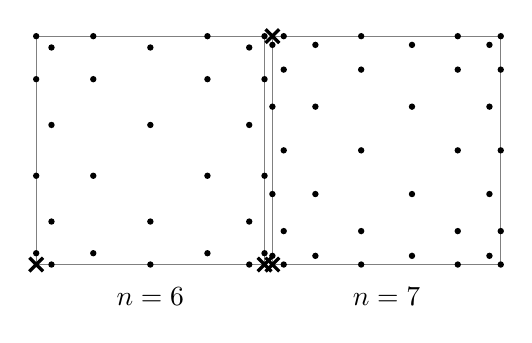
\begin{tikzpicture}[x=1.45cm,y=1.45cm]
\foreach \nn/\mm/\dx in {6/7/0,7/8/3} {
 \begin{scope}[xshift=\dx cm]
  \draw[gray] (-1,-1) rectangle (1,1);
  \foreach \jj in {0,...,\nn} {
   \foreach \kk in {0,...,\mm} {
    \pgfmathtruncatemacro{\parity}{mod(\jj+\kk,2)}
    \ifnum\parity=0
     \fill ({cos(180*\jj/\nn)},{cos(180*\kk/\mm)}) circle (0.028);
    \fi
   }
  }
  \draw[very thick] (-1.06,-1.06)--(-0.94,-0.94)
                    (-1.06,-0.94)--(-0.94,-1.06);
  \ifnum\nn=6
   \draw[very thick] (0.94,-1.06)--(1.06,-0.94)
                     (0.94,-0.94)--(1.06,-1.06);
  \else
   \draw[very thick] (-1.06,0.94)--(-0.94,1.06)
                     (-1.06,1.06)--(-0.94,0.94);
  \fi
  \node[below] at (0,-1.12) {$n=\nn$};
 \end{scope}
}
\end{tikzpicture}
\caption{The Padua points for two consecutive degrees. Dots are interpolation
points; crosses mark the two corners where the Lebesgue function attains
its maximum. The change of orientation depends only on parity.}
\label{fig:padua-nodes}
\end{figure}

Let $L_B$ be the cardinal polynomial associated with $B\in\mathcal P_n$.
The Lebesgue function and its maximum are
\[
 \lambda_n(z)=\sum_{B\in\mathcal P_n}|L_B(z)|,
 \qquad \Lambda_n=\max_{z\in[-1,1]^2}\lambda_n(z).
\]
At an interpolation point the Lebesgue function is exactly one. Away from
the points, its individual cardinal terms can reinforce each other.
For Padua interpolation the largest reinforcement occurs at the two corners
that are not interpolation points. This location was observed numerically
and posed as a question in earlier work
\cite{CaliariDeMarchiSommarivaVianello2008poster,DeMarchi2022}.
Our first result identifies these maximizers exactly.

\begin{theorem}[Location of the maximum]\label{thm:main-location}
For every integer $n\geq2$, the maximum of $\lambda_n$ on the closed square
is attained exactly at
\[
 \begin{cases}
 \{(-1,-1),(1,-1)\},&n\text{ even},\\
 \{(-1,-1),(-1,1)\},&n\text{ odd}.
 \end{cases}
\]
In particular, $\Lambda_n=\Lambda_c(n)$, where
$\Lambda_c(n):=\lambda_n(-1,-1)$.
\end{theorem}

The proof combines an analytic argument, valid for $n\geq320$, with
rigorous finite certificates for the remaining degrees. The certificates
bound the function on regions of the square; they do not infer the maximum
from a collection of sampled values. The analytic argument also uses a
separately certified constant enclosure in its quantitative estimates.
These dependencies are described in Sections~\ref{sec:argmax}
and~\ref{sec:certificates}.

Knowing the location reduces the Lebesgue constant to a single corner
value. Our second result describes that value much more precisely than
its leading growth rate. Write
\begin{equation}\label{eq:main-constants}
 a=\frac2\pi,\qquad d=\gamma+\log\frac8\pi,\qquad
 c_1=ad,\qquad b=2ac_1,\qquad c=c_1^2+\kappa,
\end{equation}
where $\gamma$ is Euler's constant and
\begin{equation}\label{eq:main-kappa}
 \kappa=\frac8\pi\int_0^1 t^2\cot\frac{\pi t}{2}
       \sum_{\substack{\ell\geq1\\\ell\text{ odd}}}
       \frac{1}{\ell(\ell^2-t^2)}\,dt.
\end{equation}
The apparent singularity at $t=1$ is canceled by the cotangent factor;
we justify convergence below.

\begin{theorem}[Sharp corner expansion]\label{thm:main-expansion}
Let $N=n+\tfrac12$. For the points \eqref{eq:nodes}, as $n\to\infty$,
\begin{equation}\label{eq:main-expansion}
 \Lambda_c(n)=\frac4{\pi^2}\log^2N+b\log N+c-\frac1N
            +O\!\left(\frac{\log N}{N^2}\right).
\end{equation}
The constants and the remainder estimate are the same for both parities.
More precisely, a finite constant $C$, independent of $n$, bounds the
absolute remainder by $C\log N/N^2$ for every integer $n\geq2$.
Consequently \eqref{eq:main-expansion} also holds for $\Lambda_n$.
\end{theorem}

The corner expansion is proved entirely analytically. Its global version
uses Theorem~\ref{thm:main-location}, with the computer-assisted dependencies
just described. No numerical fit is used to determine $b$, $c$ or the
coefficient $-1$.

\subsection{What the expansion says}
The dominant term was established by Kolomoitsev and Lomako
\cite{KolomoitsevLomako2021}:
\[
 \Lambda_n=\frac4{\pi^2}\log^2n+O(\log n).
\]
Our expansion resolves the terms hidden in that error, down to an error
smaller than $1/n$. Its leading part can be written more suggestively as
\[
 \left[\frac2\pi\left(\log N+\gamma+\log\frac8\pi\right)\right]^2
       +\kappa-\frac1N.
\]
The square comes from two one-dimensional harmonic sums. The constant
$\kappa$ measures the defect in replacing the coupled two-dimensional
corner formula by their product. The term $-1/N$ records the first
interaction between the boundary corrections and the displacement of the
two meshes. Centering at $N=n+1/2$ makes that interaction visible: a
logarithmic first correction present in the coordinate $n+1$ cancels
against the change of variable. Section~\ref{sec:asym} explains this
cancellation before turning to its estimates.

\subsection{The idea behind the maximizer proof}
A direct comparison of all the absolute cardinal terms hides useful
cancellation. Instead, we express the physical Lebesgue function as a
periodic envelope minus a nonnegative defect. The envelope is easier
to estimate. The defect measures the cancellation that is lost when one
passes to that envelope. Near a competing corner the envelope alone is
not enough: retaining the defect is what gives a strict comparison with
$\Lambda_c(n)$.

There are two different geometric tasks. Away from the two maximizing
corners, one needs a uniform positive gap. Near either maximizing corner,
no such gap can exist, because the function is continuous and equals
$\Lambda_c(n)$ at the corner itself. There we prove a strict quadratic
loss in angular coordinates. Together these arguments explain both the
maximum value and its entire equality set. The finite certificates follow
the same distinction: region bounds away from the corners, and a local
strictness argument at the corners.

\subsection{Related work and organization}
The Padua construction and its relation to generating curves and polynomial
ideals are developed in
\cite{BosCaliariDeMarchiVianelloXu2006,BosDeMarchiVianelloXu2007}.
The survey \cite{DeMarchi2022} records the corner-location question, and
\cite{BialasCiezDeMarchiSuder2026} studies geometric features of Lebesgue
functions, including numerical information about local maxima.
These questions should be distinguished from the exact global equality
set in Theorem~\ref{thm:main-location}.

Rigorous evaluation by polynomial meshes has an important earlier
foundation. Bia{\l}as-Cie{\.{z}}, Kenne, Sommariva and Vianello
\cite{Mesh2024} give certified mathematical discretization bounds for
Lebesgue constants on several domains and include Padua examples.
Such bounds control the discretization error; interval evaluation must
also control arithmetic error when they are used as numerical certificates.
Our finite completion uses strict exclusion and local corner estimates
to determine an equality set, rather than an approximation to the norm
alone. We do not claim that rigorous mesh bounds originate here.

For the related Morrow--Patterson points, Beberok, Bia{\l}as-Cie{\.{z}}
and De Marchi \cite{MorrowPatterson2026} prove quadratic growth of the
Lebesgue constant. The two node families have different stability
behavior, and their extremum questions are separate.

We first establish the exact cardinal normalization and the corner
representation. We then derive the sharp expansion, explain the geometric
comparison giving the maximizers, and describe the finite certificates.
Detailed quadrature, row and localization estimates are collected in
appendices so that the main argument can be read without following every
constant calculation.
